%Struktur: 20 min Vortrag mit 1,5 min pro Folie -> 15 Folien inkl. Titelfolie
%10 min Fragen

%%%%%%%%%%%%%%%%%%%%%%%%%%%%%%%%%%%%%%%%%%%%%%%%%%%%%%%%%%%%%%%%%%%%%%%%%%%%%%%%%%%%%%%%%%%%%%%%%%%%%%%%%%%%%%%%%%%%%%%%%%%%%%%%%%%%%%

\documentclass[colorbacktitle,inverttitle,landscape,presentation,
	english,
	aspectratio=43, %43 or 169, 1610
	accentcolor=tud9b, %tud9b (temf) or tud5b (gsce) 
]{tudbeamer}

%%additional packages(Praesentation)
%%standard:

%%language:
\usepackage[utf8]{inputenc}
\usepackage[english]{babel}
%%math:
\usepackage{amsmath}
\usepackage{caption}
\usepackage{subcaption}
%%tikz:
\usepackage{tikz}
\usetikzlibrary{patterns}
\usepackage[siunitx,americaninductors]{circuitikz}
\usepackage{siunitx}
%%pgfplots:
\usepackage{pgfplots}
\usepgfplotslibrary{groupplots}
\usepgfplotslibrary{patchplots}
\usepackage{pgfplotstable}
\pgfplotsset{compat=newest}\usepgfplotslibrary{units}
%%scaling:
\usepackage{adjustbox}
\usepackage{wrapfig,lipsum,booktabs}
%%additional packages(Praesentation)
 

%needs to come last
\usepackage{temfbeamer}

%remove TU logo from every slide but the title
\setbeamertemplate{headline}[TUD theme nologo] 

\definecolor{mygreen}{rgb}{0,0.6,0}
\definecolor{mygray}{rgb}{0.5,0.5,0.5}
\definecolor{mymauve}{rgb}{0.58,0,0.82}
\usepackage{listings}
\lstset{ %
  float=tp,
  floatplacement=tbp,
  abovecaptionskip=-5pt,
  backgroundcolor=\color{gray!25},   % choose the background color; you must add \usepackage{color} or \usepackage{xcolor}; should come as last argument
  basicstyle=\scriptsize,        % the size of the fonts that are used for the code
  breakatwhitespace=false,         % sets if automatic breaks should only happen at whitespace
  breaklines=true,                 % sets automatic line breaking
  commentstyle=\color{mygreen},    % comment style
  frame=single,	                   % adds a frame around the code
  keepspaces=true,                 % keeps spaces in text, useful for keeping indentation of code (possibly needs columns=flexible)
  keywordstyle=\color{blue},       % keyword style
  language=Python,                 % the language of the code
%  morekeywords={*,...},            % if you want to add more keywords to the set
  numbers=left,                    % where to put the line-numbers; possible values are (none, left, right)
  numbersep=5pt,                   % how far the line-numbers are from the code
  numberstyle=\tiny\color{mygray}, % the style that is used for the line-numbers
  rulecolor=\color{black},         % if not set, the frame-color may be changed on line-breaks within not-black text (e.g. comments (green here))
  showspaces=false,                % show spaces everywhere adding particular underscores; it overrides 'showstringspaces'
  showstringspaces=false,          % underline spaces within strings only
  showtabs=false,                  % show tabs within strings adding particular underscores
  stepnumber=1,                    % the step between two line-numbers. If it's 1, each line will be numbered
  stringstyle=\color{mymauve},     % string literal style
  tabsize=2,	                   % sets default tabsize to 2 spaces
}

\usepackage[absolute,overlay]{textpos}
 
 
  \setlength{\TPHorizModule}{1mm}
  \setlength{\TPVertModule}{1mm}

%set date
\date{13. August, 2018}

\newcount\WertA

\newcounter{from}
\newcounter{till}
\newcounter{onlyAt}

%%%%%%%%%%%%%%%%%%%%%%%%%%%%%%%%%%%%%%%%%%%%%%%%%%%%%%%%%%%%%%%%%%%%%%%%%%%%%%%%%%%%%%%%%%%%%%%%%%%%%%%%%%%%%%%%%%%%%%%%%%%%%%%%%%%%%%

\title{Generierung des Eingangssingals für Barrier Bucket RF Systeme and der GSI }

\subtitle{\\[0.3\baselineskip]
	Jonas Christ, Artem Moskalew, Maximilian Nolte \\
{\small Jens Harzheim, M.Sc.}\\
[0.3\baselineskip]
{\tiny Projektseminar Beschleunigertechnik}\\[0.3em]
	\mbox{\scriptsize}~}
	
\institute[TU Darmstadt | Fachbereich 18 | Institut Theorie Elektromagnetischer Felder]{Institut für Theorie Elektromagnetischer Felder, TU Darmstadt}

%%%%%%%%%%%%%%%%%%%%%%%%%%%%%%%%%%%%%%%%%%%%%%%%%%%%%%%%%%%%%%%%%%%%%%%%%%%%%%%%%%%%%%%%%%%%%%%%%%%%%%%%%%%%%%%%%%%%%%%%%%%%%%%%%%%%%%



\begin{document}
	
\begin{titleframe}
	\tudtitle[images/temf_logo.pdf]{images/temf_background.jpg} 
	%\tudtitle[images/gsce_logo.pdf]{images/gsce_background.jpg}
	\end{titleframe}
	
\begin{frame}
	\frametitle{Outline}
	\tableofcontents%[currentsection,subsectionstyle=show/show/hide]
\end{frame}
	
%%%%%%%%%%%%%%%%%%%%%%%%%%%%%%%%%%%%%%%%%%%%%%%%%%%%%%%%%%%%%%%%%%%%%%%%%%%%%%%%%%%%%%%%%%%%%%%%%%%%%%%%%%%%%%%%%%%%%%%%%%%%%%%%%%%%%%

\section{Einführung}

\subsection{Problemstellung}
\begin{frame}{Problemstellung}

\begin{itemize}
	
	\item Barrier-Bucket System \uncover<2-> {: 
		\begin{itemize}
			\item Longitudinale Manipulation der Bunches
		\end{itemize}
		}
	\item Ziel \uncover<3-> {:
		\begin{itemize}
			\item Gap Spannung in Form einer Ein-Sinus Periode
			\item Qualität das Signals
		\end{itemize}
		}
		
		%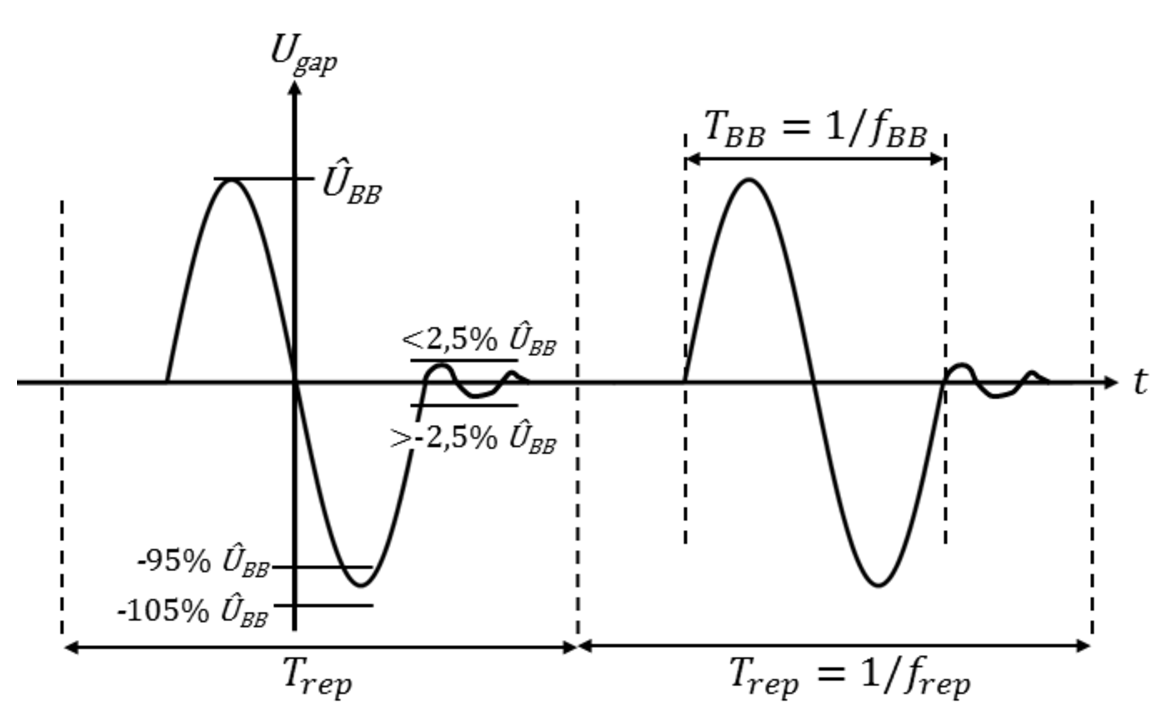
\includegraphics[scale=0.3]{slides/Problemstellung/BB_req.eps}
\end{itemize}		
\uncover<3-> {		
	\begin{picture}(10,7)
		\put(70,-90){
			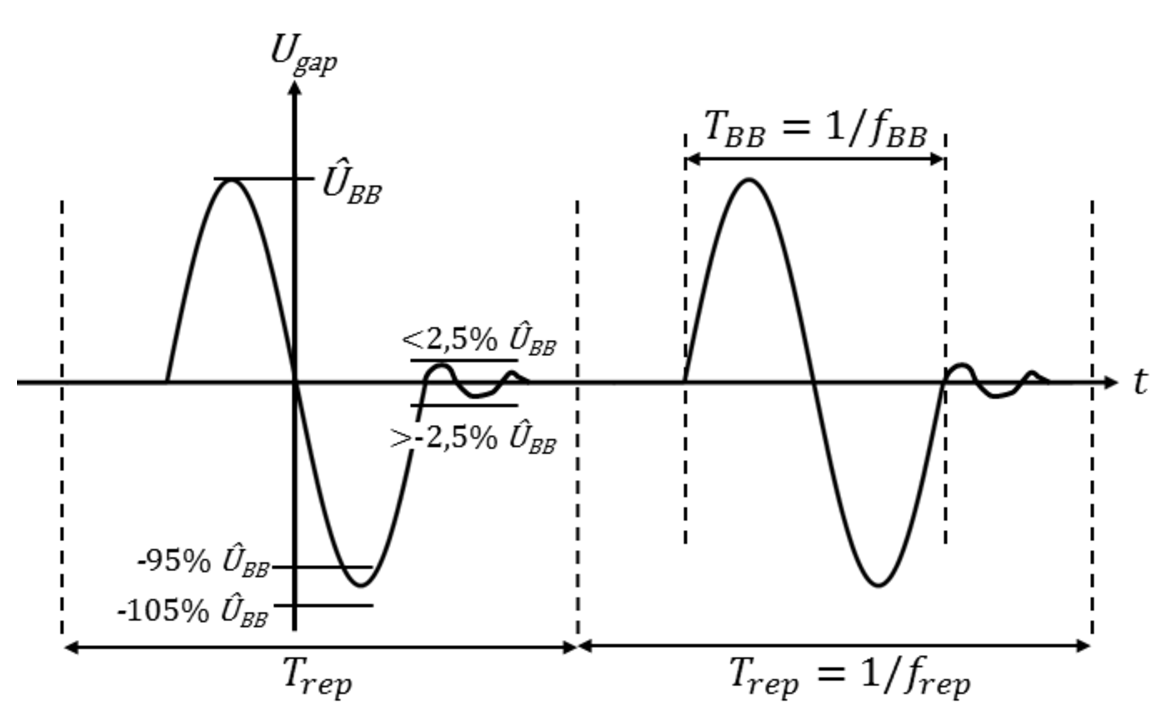
\includegraphics[scale=0.3]{slides/Problemstellung/BB_req.eps} 
		}  
	\end{picture} 
}	

\end{frame}





\subsection{Aufbau}
\begin{frame}[fragile]
\frametitle{Aufbau und Modell}

\begin{center}
		\includegraphics[scale=0.45]{slides/ResultCode/WEPVA047f2_2-eps-converted-to.pdf} 
	\end{center}
\end{frame}

\begin{frame}[fragile]
\frametitle{Aufbau und Modell}

	
	{
	\begin{itemize}
	\item Hammerstein Modell \uncover<2-> {: 
		\begin{itemize}
			\item System ist linear bis $\hat{U}_{BB} \approx 550V$
			\item Ergänzung um eine nichtlineare Vorverzerrung
			\item Potenzreihenansatz $U_?(t)=\sum_{n=1}^N a_n \left[ U_{in}(t) \right]^n$
		\end{itemize}
		}
	\item Zielsetzung \uncover<3-> {:
		\begin{itemize}
			\item Parameter $a_n$ der Kennlinie zubestimmen
		\end{itemize}
		}
	 \end{itemize}
	}
	\centering
	\begin{picture}(100,70)
		\put(15,5){
			\includegraphics[scale=1.0]{slides/ResultCode/Slide1.eps} 
		}
	\end{picture}
%\begin{picture}(100,70)
%		\put(15,0){
%			\includegraphics[scale=1.0]{slides/ResultCode/Slide2.eps} 
%		}  
%	\end{picture}
\end{frame}



\section{Code}

\WertA=1
<<<<<<< HEAD
\section{Design}
\subsection{Blöcke}


\begin{frame}[fragile]
\ifnum\WertA=1
\frametitle{Code: Das Design}
\else
\frametitle{Code: Evaluierung}
\fi

%\only<1>
%	{ 
%\framebox{   %   % just so you can see where the "picture" is

\setcounter{onlyAt}{0}

\ifnum\WertA=1

\setcounter{onlyAt}{\value{onlyAt}+1}
\only<\value{onlyAt}>
{
	\begin{center}
		\includegraphics[scale=0.45]{slides/ResultCode/WEPVA047f2_2-eps-converted-to.pdf} 
	\end{center}
}

\setcounter{onlyAt}{\value{onlyAt}+1}
\only<\value{onlyAt}>
	{
	\begin{picture}(100,70)
		\put(15,0){
			\includegraphics[scale=1.0]{slides/ResultCode/Slide1.eps} 
		}  
	\end{picture} 
	}
\fi
		
\setcounter{onlyAt}{\value{onlyAt}+1}
\only<\value{onlyAt}>
	{
	\begin{picture}(100,70)
		\put(15,0){
			\includegraphics[scale=1.0]{slides/ResultCode/Slide2.eps} 
		}  
	\end{picture} 
	}
	


\ifnum\WertA=1 \setcounter{from}{\value{onlyAt}+1} \setcounter{till}{\value{onlyAt}+1} \else \setcounter{from}{\value{onlyAt}+1} \setcounter{till}{\value{onlyAt}+2} \fi	
\only<\value{from} - \value{till}> 
	{
	\begin{picture}(100,70)
		\put(15,0){
			\includegraphics[scale=1.0]{slides/ResultCode/Slide3.eps} 
		}  
	\end{picture} 
	\lstinputlisting[firstline=1,lastline=1]{slides/ResultCode/file.txt} 
	}	
	
\ifnum\WertA=2
	\setcounter{onlyAt}{\value{from} + 1}
	\only<\value{onlyAt}>
	{
		\begin{textblock}{20}(80,50)
    		\includegraphics[height=3.5cm, width=4.5cm ]{slides/ResultCode/plots/Uout_ideal.pdf} 
		\end{textblock}	
	} 	
\fi	
\setcounter{onlyAt}{\value{till}}


\ifnum\WertA=1 \setcounter{from}{\value{onlyAt}+1} \setcounter{till}{\value{onlyAt}+1} \else \setcounter{from}{\value{onlyAt}+1} \setcounter{till}{\value{onlyAt}+2} \fi	
\only<\value{from} - \value{till}> 
	{
	\begin{picture}(100,70)
		\put(15,0){
			\includegraphics[scale=1.0]{slides/ResultCode/Slide4.eps} 
		}  
	\end{picture} 
	\lstinputlisting[firstline=1,lastline=2]{slides/ResultCode/file.txt} 
	}
	
\ifnum\WertA=2
	\setcounter{onlyAt}{\value{from} + 1}
	\only<\value{onlyAt}>
	{
		\begin{textblock}{20}(93,50)
    		\includegraphics[ width=3.5cm, height=3.1cm ]{slides/ResultCode/plots/H_p.pdf} 
		\end{textblock}			
		\begin{textblock}{20}(61,50)
    		\includegraphics[ width=3.5cm, height=3.1cm]{slides/ResultCode/plots/H_a.pdf} 
		\end{textblock}	
		
	} 	 
\fi	
\setcounter{onlyAt}{\value{till}} 

\setcounter{onlyAt}{\value{onlyAt}+1}
\only<\value{onlyAt}>
	{
	\begin{picture}(100,70)
		\put(15,0){
			\includegraphics[scale=1.0]{slides/ResultCode/Slide5.eps} 
		}  
	\end{picture} 
	\lstinputlisting[firstline=1,lastline=3]{slides/ResultCode/file.txt} 
	}	
	
\setcounter{onlyAt}{\value{onlyAt}+1}
\only<\value{onlyAt}>
	{
	\begin{picture}(100,70)
		\put(15,0){
			\includegraphics[scale=1.0]{slides/ResultCode/Slide5-1.eps} 
		}  
	\end{picture} 
	\lstinputlisting[firstline=1,lastline=3]{slides/ResultCode/file.txt} 
	}
	
\ifnum\WertA=2
	\setcounter{from}{\value{onlyAt}} 
	\setcounter{till}{\value{onlyAt}+2}
	\only<\value{from} - \value{till}>
	{
		\begin{textblock}{20}(80,50)
    		\includegraphics[height=3.5cm, width=4.5cm ]{slides/ResultCode/plots/U_quest_ideal.pdf} 
		\end{textblock}	
	} 
\fi	

\setcounter{onlyAt}{\value{onlyAt}+1}
\only<\value{onlyAt}>
{
	\begin{picture}(100,70)
		\put(15,0)
		{
			\includegraphics[scale=1.0]{slides/ResultCode/Slide6.eps} 
		}  
	\end{picture} 
	\lstinputlisting[firstline=1,lastline=3]{slides/ResultCode/file.txt} 
}

\setcounter{onlyAt}{\value{onlyAt}+1}
\only<\value{onlyAt}>
{
	\begin{picture}(100,70)
		\put(15,0)
		{
			\includegraphics[scale=1.0]{slides/ResultCode/Slide7.eps} 
		}
	\end{picture} 	
	\lstinputlisting[firstline=1,lastline=4]{slides/ResultCode/file.txt} 	
}	

\setcounter{onlyAt}{\value{onlyAt}+1}
\only<\value{onlyAt}>
{
	\begin{picture}(100,70)
		\put(15,0)
		{
			\includegraphics[scale=1.0]{slides/ResultCode/Slide7.eps} 
		}
	\end{picture} 	
	\lstinputlisting[firstline=1,lastline=5]{slides/ResultCode/file.txt} 		

}

\ifnum\WertA=1 \setcounter{from}{\value{onlyAt}+1} \setcounter{till}{\value{onlyAt}+1} \else \setcounter{from}{\value{onlyAt}+1} \setcounter{till}{\value{onlyAt}+3} \fi	
\only<\value{from} - \value{till}> 
{
	\begin{picture}(100,70)
		\put(15,0)
		{
			\includegraphics[scale=1.0]{slides/ResultCode/Slide8.eps} 
		}
	\end{picture} 	
	\lstinputlisting[firstline=1,lastline=5]{slides/ResultCode/file.txt} 		

}

\ifnum\WertA=2
	\setcounter{onlyAt}{\value{from}+1}
	\only<\value{onlyAt}>
	{
		\begin{textblock}{20}(80,50)
    		\includegraphics[height=3.5cm, width=4.5cm ]{slides/ResultCode/plots/Uout_measured.pdf} 
		\end{textblock}	
	} 
	\setcounter{onlyAt}{\value{from}+2}
	\only<\value{onlyAt}>
	{
		\begin{textblock}{20}(80,50)
    		\includegraphics[height=3.5cm, width=4.5cm ]{slides/ResultCode/plots/Uout_measured_cut.pdf} 
		\end{textblock}	
	} 
\fi
\setcounter{onlyAt}{\value{till}} 
 
\ifnum\WertA=1 \setcounter{from}{\value{onlyAt}+1} \setcounter{till}{\value{onlyAt}+1} \else \setcounter{from}{\value{onlyAt}+1} \setcounter{till}{\value{onlyAt}+2} \fi	
\only<\value{from} - \value{till}> 
{
	\begin{picture}(100,70)
		\put(15,0)
		{
			\includegraphics[scale=1.0]{slides/ResultCode/Slide9.eps} 
		}  
	\end{picture} 
	\lstinputlisting[firstline=1,lastline=6]{slides/ResultCode/file.txt} 
}	

\ifnum\WertA=2
	\setcounter{onlyAt}{\value{from} + 1}
	\only<\value{onlyAt}>
	{
		\begin{textblock}{20}(80,50)
    		\includegraphics[height=3.5cm, width=4.5cm ]{slides/ResultCode/plots/U_quest_measured.pdf} 
		\end{textblock}	
	}
\fi
\setcounter{onlyAt}{\value{till}} 
	
\setcounter{onlyAt}{\value{onlyAt}+1}
\only<\value{onlyAt}>
{
	\begin{picture}(100,70)
		\put(15,0){
			\includegraphics[scale=1.0]{slides/ResultCode/Slide10.eps} 
		}  
	\end{picture} 
	\lstinputlisting[firstline=1,lastline=7]{slides/ResultCode/file.txt} 
}



\ifnum\WertA=1 \setcounter{from}{\value{onlyAt}+1} \setcounter{till}{\value{onlyAt}+1} \else \setcounter{from}{\value{onlyAt}+1} \setcounter{till}{\value{onlyAt}+2} \fi	
\only<\value{from} - \value{till}> 
{
	\begin{picture}(100,70)
		\put(15,0)
		{
			\includegraphics[scale=1.0]{slides/ResultCode/Slide11.eps} 
		}  
	\end{picture} 
	\lstinputlisting[firstline=1,lastline=8]{slides/ResultCode/file.txt} 
}

\ifnum\WertA=2
	\setcounter{onlyAt}{\value{from} + 1}
	\only<\value{onlyAt}>
	{
		\begin{textblock}{20}(80,50)
    		\includegraphics[height=3.5cm, width=4.5cm ]{slides/ResultCode/plots/K.pdf} 
		\end{textblock}	
	} 
\fi	
\setcounter{onlyAt}{\value{till}}	

\setcounter{onlyAt}{\value{onlyAt}+1}
\only<\value{onlyAt}>
{
	\begin{picture}(100,70)
		\put(15,0)
		{
			\includegraphics[scale=1.0]{slides/ResultCode/Slide12-0.eps} 
		}  
	\end{picture} 
	\lstinputlisting[firstline=1,lastline=8]{slides/ResultCode/file.txt} 
}
	
\setcounter{onlyAt}{\value{onlyAt}+1}
\only<\value{onlyAt}>
{
	\begin{picture}(100,70)
		\put(15,0)
		{
			\includegraphics[scale=1.0]{slides/ResultCode/Slide12-01.eps} 
		}  
	\end{picture} 
	\lstinputlisting[firstline=1,lastline=8]{slides/ResultCode/file.txt} 
}
	
\setcounter{onlyAt}{\value{onlyAt}+1}
\only<\value{onlyAt}>
{
	\begin{picture}(100,70)
		\put(15,0)
		{
			\includegraphics[scale=1.0]{slides/ResultCode/Slide12.eps} 
		}  
	\end{picture} 
	\lstinputlisting[firstline=1,lastline=9]{slides/ResultCode/file.txt} 
}
	
\setcounter{onlyAt}{\value{onlyAt}+1}
\only<\value{onlyAt}>
{
	\begin{picture}(100,70)
		\put(15,0)
		{
			\includegraphics[scale=1.0]{slides/ResultCode/Slide13-0.eps} 
		}  
	\end{picture} 
	\lstinputlisting[firstline=1,lastline=9]{slides/ResultCode/file.txt} 
}

\setcounter{onlyAt}{\value{onlyAt}+1}
\only<\value{onlyAt}>
{
	\begin{picture}(100,70)
		\put(15,0)
		{
			\includegraphics[scale=1.0]{slides/ResultCode/Slide13-01.eps} 
		}  
	\end{picture} 
	\lstinputlisting[firstline=1,lastline=10]{slides/ResultCode/file.txt} 
}
	
\setcounter{onlyAt}{\value{onlyAt}+1}
\only<\value{onlyAt}>
{
	\begin{picture}(100,70)
		\put(15,0)
		{
			\includegraphics[scale=1.0]{slides/ResultCode/Slide13.eps} 
		}  
	\end{picture} 
	\lstinputlisting[firstline=1,lastline=11]{slides/ResultCode/file.txt} 
}

  
%	\begin{figure}[t]
%	
%%	
%	\end{figure}	
	%}
%\only<2>{ \lstinputlisting[firstline=1,lastline=2]{slides/ResultCode/file.txt} }
%\only<3>{ \lstinputlisting[firstline=1,lastline=3]{slides/ResultCode/file.txt} }
%\only<4>{ \lstinputlisting[firstline=1,lastline=4]{slides/ResultCode/file.txt} }
%\only<5>{ \lstinputlisting[firstline=1,lastline=5]{slides/ResultCode/file.txt} }
%\only<6>{ \lstinputlisting[firstline=1,lastline=6]{slides/ResultCode/file.txt} }
%\only<7>{ \lstinputlisting[firstline=1,lastline=7]{slides/ResultCode/file.txt} }
%\only<8>{ \lstinputlisting[firstline=1,lastline=8]{slides/ResultCode/file.txt} }
%\only<9>{ \lstinputlisting[firstline=1,lastline=9]{slides/ResultCode/file.txt} }
%\only<10>{ \lstinputlisting[firstline=1,lastline=10]{slides/ResultCode/file.txt} }


\end{frame}





%\subsection{Vorgehensweise}
\subsection{Test Driven Development}
\begin{frame}
\frametitle{\textbf{T}est \textbf{D}riven \textbf{D}evelopment}

\onslide<2->{
\begin{itemize}
	\onslide<2->{\item 27 Unit Tests}
	\onslide<3->{\item 4 System Tests}
\end{itemize}
}
\onslide<4->{Vorteile:
\onslide<5->{
\begin{itemize}
	\onslide<5->{\item Ermöglichen:	
	\begin{itemize}
		\onslide<5->{\item inkrementierende Code-Anpassungen}
		\onslide<6->{\item verteiltes Debuggen ohne den Messaufbau}	
	\end{itemize}		
 	}
	\onslide<7->{\item Zwingen zum modularen Code-Design}
	\onslide<8->{\item Erleichtern das Migrieren der Funktionen aus anderen Sprachen }
\end{itemize}
}
}
 

\onslide<9->{Nachteile:
\onslide<10->{
\begin{itemize}
	\onslide<10->{\item Extra Aufwand: Mehr Code zu debuggen}
\end{itemize}
}
}
 
 

\end{frame}

\subsection{MockSystem}
=======
\subsection{Design}


\begin{frame}[fragile]
\ifnum\WertA=1
\frametitle{Code: Das Design}
\else
\frametitle{Code: Evaluierung}
\fi

%\only<1>
%	{ 
%\framebox{   %   % just so you can see where the "picture" is

\setcounter{onlyAt}{0}

\ifnum\WertA=1

\setcounter{onlyAt}{\value{onlyAt}+1}
\only<\value{onlyAt}>
{
	\begin{center}
		\includegraphics[scale=0.45]{slides/ResultCode/WEPVA047f2_2-eps-converted-to.pdf} 
	\end{center}
}

\setcounter{onlyAt}{\value{onlyAt}+1}
\only<\value{onlyAt}>
	{
	\begin{picture}(100,70)
		\put(15,0){
			\includegraphics[scale=1.0]{slides/ResultCode/Slide1.eps} 
		}  
	\end{picture} 
	}
\fi
		
\setcounter{onlyAt}{\value{onlyAt}+1}
\only<\value{onlyAt}>
	{
	\begin{picture}(100,70)
		\put(15,0){
			\includegraphics[scale=1.0]{slides/ResultCode/Slide2.eps} 
		}  
	\end{picture} 
	}
	


\ifnum\WertA=1 \setcounter{from}{\value{onlyAt}+1} \setcounter{till}{\value{onlyAt}+1} \else \setcounter{from}{\value{onlyAt}+1} \setcounter{till}{\value{onlyAt}+2} \fi	
\only<\value{from} - \value{till}> 
	{
	\begin{picture}(100,70)
		\put(15,0){
			\includegraphics[scale=1.0]{slides/ResultCode/Slide3.eps} 
		}  
	\end{picture} 
	\lstinputlisting[firstline=1,lastline=1]{slides/ResultCode/file.txt} 
	}	
	
\ifnum\WertA=2
	\setcounter{onlyAt}{\value{from} + 1}
	\only<\value{onlyAt}>
	{
		\begin{textblock}{20}(80,50)
    		\includegraphics[height=3.5cm, width=4.5cm ]{slides/ResultCode/plots/Uout_ideal.pdf} 
		\end{textblock}	
	} 	
\fi	
\setcounter{onlyAt}{\value{till}}


\ifnum\WertA=1 \setcounter{from}{\value{onlyAt}+1} \setcounter{till}{\value{onlyAt}+1} \else \setcounter{from}{\value{onlyAt}+1} \setcounter{till}{\value{onlyAt}+2} \fi	
\only<\value{from} - \value{till}> 
	{
	\begin{picture}(100,70)
		\put(15,0){
			\includegraphics[scale=1.0]{slides/ResultCode/Slide4.eps} 
		}  
	\end{picture} 
	\lstinputlisting[firstline=1,lastline=2]{slides/ResultCode/file.txt} 
	}
	
\ifnum\WertA=2
	\setcounter{onlyAt}{\value{from} + 1}
	\only<\value{onlyAt}>
	{
		\begin{textblock}{20}(93,50)
    		\includegraphics[ width=3.5cm, height=3.1cm ]{slides/ResultCode/plots/H_p.pdf} 
		\end{textblock}			
		\begin{textblock}{20}(61,50)
    		\includegraphics[ width=3.5cm, height=3.1cm]{slides/ResultCode/plots/H_a.pdf} 
		\end{textblock}	
		
	} 	 
\fi	
\setcounter{onlyAt}{\value{till}} 

\setcounter{onlyAt}{\value{onlyAt}+1}
\only<\value{onlyAt}>
	{
	\begin{picture}(100,70)
		\put(15,0){
			\includegraphics[scale=1.0]{slides/ResultCode/Slide5.eps} 
		}  
	\end{picture} 
	\lstinputlisting[firstline=1,lastline=3]{slides/ResultCode/file.txt} 
	}	
	
\setcounter{onlyAt}{\value{onlyAt}+1}
\only<\value{onlyAt}>
	{
	\begin{picture}(100,70)
		\put(15,0){
			\includegraphics[scale=1.0]{slides/ResultCode/Slide5-1.eps} 
		}  
	\end{picture} 
	\lstinputlisting[firstline=1,lastline=3]{slides/ResultCode/file.txt} 
	}
	
\ifnum\WertA=2
	\setcounter{from}{\value{onlyAt}} 
	\setcounter{till}{\value{onlyAt}+2}
	\only<\value{from} - \value{till}>
	{
		\begin{textblock}{20}(80,50)
    		\includegraphics[height=3.5cm, width=4.5cm ]{slides/ResultCode/plots/U_quest_ideal.pdf} 
		\end{textblock}	
	} 
\fi	

\setcounter{onlyAt}{\value{onlyAt}+1}
\only<\value{onlyAt}>
{
	\begin{picture}(100,70)
		\put(15,0)
		{
			\includegraphics[scale=1.0]{slides/ResultCode/Slide6.eps} 
		}  
	\end{picture} 
	\lstinputlisting[firstline=1,lastline=3]{slides/ResultCode/file.txt} 
}

\setcounter{onlyAt}{\value{onlyAt}+1}
\only<\value{onlyAt}>
{
	\begin{picture}(100,70)
		\put(15,0)
		{
			\includegraphics[scale=1.0]{slides/ResultCode/Slide7.eps} 
		}
	\end{picture} 	
	\lstinputlisting[firstline=1,lastline=4]{slides/ResultCode/file.txt} 	
}	

\setcounter{onlyAt}{\value{onlyAt}+1}
\only<\value{onlyAt}>
{
	\begin{picture}(100,70)
		\put(15,0)
		{
			\includegraphics[scale=1.0]{slides/ResultCode/Slide7.eps} 
		}
	\end{picture} 	
	\lstinputlisting[firstline=1,lastline=5]{slides/ResultCode/file.txt} 		

}

\ifnum\WertA=1 \setcounter{from}{\value{onlyAt}+1} \setcounter{till}{\value{onlyAt}+1} \else \setcounter{from}{\value{onlyAt}+1} \setcounter{till}{\value{onlyAt}+3} \fi	
\only<\value{from} - \value{till}> 
{
	\begin{picture}(100,70)
		\put(15,0)
		{
			\includegraphics[scale=1.0]{slides/ResultCode/Slide8.eps} 
		}
	\end{picture} 	
	\lstinputlisting[firstline=1,lastline=5]{slides/ResultCode/file.txt} 		

}

\ifnum\WertA=2
	\setcounter{onlyAt}{\value{from}+1}
	\only<\value{onlyAt}>
	{
		\begin{textblock}{20}(80,50)
    		\includegraphics[height=3.5cm, width=4.5cm ]{slides/ResultCode/plots/Uout_measured.pdf} 
		\end{textblock}	
	} 
	\setcounter{onlyAt}{\value{from}+2}
	\only<\value{onlyAt}>
	{
		\begin{textblock}{20}(80,50)
    		\includegraphics[height=3.5cm, width=4.5cm ]{slides/ResultCode/plots/Uout_measured_cut.pdf} 
		\end{textblock}	
	} 
\fi
\setcounter{onlyAt}{\value{till}} 
 
\ifnum\WertA=1 \setcounter{from}{\value{onlyAt}+1} \setcounter{till}{\value{onlyAt}+1} \else \setcounter{from}{\value{onlyAt}+1} \setcounter{till}{\value{onlyAt}+2} \fi	
\only<\value{from} - \value{till}> 
{
	\begin{picture}(100,70)
		\put(15,0)
		{
			\includegraphics[scale=1.0]{slides/ResultCode/Slide9.eps} 
		}  
	\end{picture} 
	\lstinputlisting[firstline=1,lastline=6]{slides/ResultCode/file.txt} 
}	

\ifnum\WertA=2
	\setcounter{onlyAt}{\value{from} + 1}
	\only<\value{onlyAt}>
	{
		\begin{textblock}{20}(80,50)
    		\includegraphics[height=3.5cm, width=4.5cm ]{slides/ResultCode/plots/U_quest_measured.pdf} 
		\end{textblock}	
	}
\fi
\setcounter{onlyAt}{\value{till}} 
	
\setcounter{onlyAt}{\value{onlyAt}+1}
\only<\value{onlyAt}>
{
	\begin{picture}(100,70)
		\put(15,0){
			\includegraphics[scale=1.0]{slides/ResultCode/Slide10.eps} 
		}  
	\end{picture} 
	\lstinputlisting[firstline=1,lastline=7]{slides/ResultCode/file.txt} 
}



\ifnum\WertA=1 \setcounter{from}{\value{onlyAt}+1} \setcounter{till}{\value{onlyAt}+1} \else \setcounter{from}{\value{onlyAt}+1} \setcounter{till}{\value{onlyAt}+2} \fi	
\only<\value{from} - \value{till}> 
{
	\begin{picture}(100,70)
		\put(15,0)
		{
			\includegraphics[scale=1.0]{slides/ResultCode/Slide11.eps} 
		}  
	\end{picture} 
	\lstinputlisting[firstline=1,lastline=8]{slides/ResultCode/file.txt} 
}

\ifnum\WertA=2
	\setcounter{onlyAt}{\value{from} + 1}
	\only<\value{onlyAt}>
	{
		\begin{textblock}{20}(80,50)
    		\includegraphics[height=3.5cm, width=4.5cm ]{slides/ResultCode/plots/K.pdf} 
		\end{textblock}	
	} 
\fi	
\setcounter{onlyAt}{\value{till}}	

\setcounter{onlyAt}{\value{onlyAt}+1}
\only<\value{onlyAt}>
{
	\begin{picture}(100,70)
		\put(15,0)
		{
			\includegraphics[scale=1.0]{slides/ResultCode/Slide12-0.eps} 
		}  
	\end{picture} 
	\lstinputlisting[firstline=1,lastline=8]{slides/ResultCode/file.txt} 
}
	
\setcounter{onlyAt}{\value{onlyAt}+1}
\only<\value{onlyAt}>
{
	\begin{picture}(100,70)
		\put(15,0)
		{
			\includegraphics[scale=1.0]{slides/ResultCode/Slide12-01.eps} 
		}  
	\end{picture} 
	\lstinputlisting[firstline=1,lastline=8]{slides/ResultCode/file.txt} 
}
	
\setcounter{onlyAt}{\value{onlyAt}+1}
\only<\value{onlyAt}>
{
	\begin{picture}(100,70)
		\put(15,0)
		{
			\includegraphics[scale=1.0]{slides/ResultCode/Slide12.eps} 
		}  
	\end{picture} 
	\lstinputlisting[firstline=1,lastline=9]{slides/ResultCode/file.txt} 
}
	
\setcounter{onlyAt}{\value{onlyAt}+1}
\only<\value{onlyAt}>
{
	\begin{picture}(100,70)
		\put(15,0)
		{
			\includegraphics[scale=1.0]{slides/ResultCode/Slide13-0.eps} 
		}  
	\end{picture} 
	\lstinputlisting[firstline=1,lastline=9]{slides/ResultCode/file.txt} 
}

\setcounter{onlyAt}{\value{onlyAt}+1}
\only<\value{onlyAt}>
{
	\begin{picture}(100,70)
		\put(15,0)
		{
			\includegraphics[scale=1.0]{slides/ResultCode/Slide13-01.eps} 
		}  
	\end{picture} 
	\lstinputlisting[firstline=1,lastline=10]{slides/ResultCode/file.txt} 
}
	
\setcounter{onlyAt}{\value{onlyAt}+1}
\only<\value{onlyAt}>
{
	\begin{picture}(100,70)
		\put(15,0)
		{
			\includegraphics[scale=1.0]{slides/ResultCode/Slide13.eps} 
		}  
	\end{picture} 
	\lstinputlisting[firstline=1,lastline=11]{slides/ResultCode/file.txt} 
}

  
%	\begin{figure}[t]
%	
%%	
%	\end{figure}	
	%}
%\only<2>{ \lstinputlisting[firstline=1,lastline=2]{slides/ResultCode/file.txt} }
%\only<3>{ \lstinputlisting[firstline=1,lastline=3]{slides/ResultCode/file.txt} }
%\only<4>{ \lstinputlisting[firstline=1,lastline=4]{slides/ResultCode/file.txt} }
%\only<5>{ \lstinputlisting[firstline=1,lastline=5]{slides/ResultCode/file.txt} }
%\only<6>{ \lstinputlisting[firstline=1,lastline=6]{slides/ResultCode/file.txt} }
%\only<7>{ \lstinputlisting[firstline=1,lastline=7]{slides/ResultCode/file.txt} }
%\only<8>{ \lstinputlisting[firstline=1,lastline=8]{slides/ResultCode/file.txt} }
%\only<9>{ \lstinputlisting[firstline=1,lastline=9]{slides/ResultCode/file.txt} }
%\only<10>{ \lstinputlisting[firstline=1,lastline=10]{slides/ResultCode/file.txt} }


\end{frame}





\subsection{Vorgehensweise}
\begin{frame}
\frametitle{Code: Vorgehensweise}

\only<2->{
\begin{itemize}
	\only<2->{\item Refactoring / Anpassung der Matlab-Funktionen an unser Design}
	\only<3->{\item Portierung der Matlab-Funktionen nach Python}
	\only<4->{\item Überprüfung der portierten Funktionen mithilfe von \textbf{TDD}}
	\only<5->{\item Erweiterung der Blöcken mit \texttt{adjust\_H}   und \texttt{adjust\_a}  }
	\only<6->{\item Neue Klassen \texttt{signale\_class} und \texttt{transfer\_function\_class}} 
\end{itemize}
}
 

\end{frame}

\begin{frame}
\frametitle{\textbf{T}est \textbf{D}riven \textbf{D}evelopment}

\onslide<2->{
\begin{itemize}
	\onslide<2->{\item 27 Unit Tests}
	\onslide<3->{\item 4 System Tests}
\end{itemize}
}
\onslide<4->{Vorteile:
\onslide<5->{
\begin{itemize}
	\onslide<5->{\item Ermöglichen:	
	\begin{itemize}
		\onslide<5->{\item inkrementierende Code-Anpassungen}
		\onslide<6->{\item verteiltes Debuggen ohne den Messaufbau}	
	\end{itemize}		
 	}
	\onslide<7->{\item Zwingen zum modularen Code-Design}
	\onslide<8->{\item Erleichtern das Migrieren der Funktionen aus anderen Sprachen }
\end{itemize}
}
}
 

\onslide<9->{Nachteile:
\onslide<10->{
\begin{itemize}
	\onslide<10->{\item Extra Aufwand: Mehr Code zu debuggen}
\end{itemize}
}
}
 
 

\end{frame}

>>>>>>> b169fb0089a2e9f292516d071d31fc35f2a151dd
\begin{frame}
\frametitle{Das Mock-System}

\onslide<2->{
\begin{itemize}
	\onslide<1->{\item Wird genutzt, wenn mit Geräten kommuniziert wird:	
	\begin{itemize}
		\item \texttt{mock\_system.write\_to\_AWG}
		\item \texttt{mock\_system.read\_from\_DSO}
	\end{itemize}		
 	}
	\onslide<3->{\item Simuliert das Verhalten des Messaufbaus nach dem Hammerstein Model}
\end{itemize}
	
}


\onslide<4->{Vorteile:
\onslide<5->{
\begin{itemize}
	\onslide<5->{\item Ermöglicht:	
	\begin{itemize}
			\onslide<5->{\item Unit Tests von Bausteinen, in den Gerätekommunikation stattfindet }
			\onslide<6->{\item System Tests }	
			\onslide<7->{\item Testen von Randfällen}
	\end{itemize}		
 	}
	\onslide<8->{\item Hilft das System besser zu verstehen }
\end{itemize}
}
} 

\onslide<9->{Nachteile:
\onslide<9->{
\begin{itemize}
	\onslide<9->{\item Extra Aufwand: mehr Code zu debuggen}
\end{itemize}
}
}
 
 

\end{frame}


\section{Optimierung}
\subsection{Optimierung der Übertragungsfunktion}
\begin{frame}{Optimierung der Übertragungsfunktion}

\uncover<2->{
Idee: Iterative Anpassung mit
\begin{align*}
			\underline{H}^{i+1} \left( \omega \right) = \underline{H}^{i} \left( \omega \right) \left( 1+ \sigma_H \cdot \left( \frac{\underline{U}_{out,\mathrm{mess}}^{i} \left( \omega \right) }{\underline{U}_{out,\mathrm{ideal}}^{i} \left( \omega \right) } -1 \right) \right) 
		\end{align*}
mit $ \sigma_H $ als Schrittweite.
}
\begin{itemize}
\uncover<3->{
\item Fokus auf Optimierung des Betrags nach ersten Messungen mit Phasenanpassung
}
\end{itemize}

\uncover<4>{
	\begin{picture}(0, -40)
	\put(120, -30){
		\includegraphics[scale=0.7]{slides/adjust_H/adjust_H_mock.png}	
	}
\end{picture}	
}

%\uncover<2-4, 5->{
%	\begin{picture}(0,70)
%		\put(15,5){
%			\includegraphics[scale=1.0]{slides/Problemstellung/Slide1.eps} 
%		}
%	\end{picture}
%	}
%

\end{frame}




\begin{frame}{Optimierung der Übertragungsfunktion}

%\uncover<1-> {
%\begin{align*}
%			\underline{H}^{i+1} \left( \omega \right) = \underline{H}^{i} \left( \omega \right) \left( 1+ \sigma_H \cdot \left( \frac{\underline{U}_{out,\mathrm{mess}}^{i} \left( \omega \right) }{\underline{U}_{out,\mathrm{ideal}}^{i} \left( \omega \right) } -1 \right) \right) 
%		\end{align*}
%}

\uncover<2->{
Fehlerquellen:
}
\begin{itemize}
	\uncover<3->{
		\item Diskretisierungsfehler durch die FFT
	}		
	\uncover<4->{
		\item Interpolationsfehler bei Auswertung des Korrektur-Terms
	}
	\uncover<5->{
		\item Rauscheinflüsse bei Messungen
	}	
\end{itemize}

\uncover<7->{
Erste Lösungsansätze:
}

\begin{itemize}
	\uncover<8->{
		\item Ignorieren kleiner Beträge in Spektren der Signale
	}
	\uncover<9->{
		\item Ignorieren großer Korrektur-Terme
	}
	\uncover<10->{
		\item \textit{Zero-Padding}
	}
\end{itemize}
\uncover<11->{
$\longrightarrow$ Simulation der komplexen Optimierung am Mock-System
}
\uncover<14->{
\\ \textbf{Ergebnis}: noch nicht ausgereift
}

%
\uncover<6>{
	\begin{picture}(0, -90)
	\put(170, -38){
		\includegraphics[scale=0.6]{slides/adjust_H/adjust_H_spectre.png}	
	}
\end{picture}	
}


\uncover<12>{
	\begin{picture}(0, -40)
	\put(145, 88){
		\includegraphics[scale=0.5]{slides/adjust_H/adjust_H_quality.png}	
	}
\end{picture}	
}

%
\uncover<13>{
	\begin{picture}(0, -80)
	\put(177, 70){
		\includegraphics[scale=0.5]{slides/adjust_H/adjust_H_high_frequencies.png}	
	}
\end{picture}	
}


\end{frame}





\subsection{Optimierung der Kennlinie}
% This file was created by matplotlib2tikz v0.6.17.
\begin{tikzpicture}

\definecolor{color0}{rgb}{0.12156862745098,0.466666666666667,0.705882352941177}
\definecolor{color1}{rgb}{1,0.498039215686275,0.0549019607843137}

\begin{axis}[
xlabel={$U_{in}$ in \si{\milli \volt}},
ylabel={$U_{?}$ in \si{\milli \volt}},
xmin=-330, xmax=330,
ymin=-703.9464559176, ymax=610.6443744396,
width=\figurewidth,
height=\figureheight,
tick align=outside,
tick pos=left,
x grid style={white!69.01960784313725!black},
y grid style={white!69.01960784313725!black},
legend cell align={left},
legend entries={{K0},{K1}},
legend style={at={(0.03,0.97)}, anchor=north west, draw=white!80.0!black}
]
\addlegendimage{no markers, color0}
\addlegendimage{no markers, color1}
\addplot [semithick, color0]
table {%
-300 -355.073268737
-299 -355.413336321
-298 -355.737870278
-297 -356.046924387
-296 -356.340552425
-295 -356.618808173
-294 -356.881745408
-293 -357.129417909
-292 -357.361879456
-291 -357.579183826
-290 -357.781384799
-289 -357.968536153
-288 -358.140691667
-287 -358.29790512
-286 -358.44023029
-285 -358.567720957
-284 -358.680430898
-283 -358.778413893
-282 -358.861723721
-281 -358.93041416
-280 -358.984538988
-279 -359.024151986
-278 -359.04930693
-277 -359.060057601
-276 -359.056457777
-275 -359.038561236
-274 -359.006421757
-273 -358.96009312
-272 -358.899629102
-271 -358.825083483
-270 -358.736510041
-269 -358.633962555
-268 -358.517494804
-267 -358.387160566
-266 -358.24301362
-265 -358.085107746
-264 -357.913496721
-263 -357.728234324
-262 -357.529374334
-261 -357.316970531
-260 -357.091076691
-259 -356.851746596
-258 -356.599034022
-257 -356.332992749
-256 -356.053676556
-255 -355.761139221
-254 -355.455434522
-253 -355.13661624
-252 -354.804738152
-251 -354.459854038
-250 -354.102017675
-249 -353.731282843
-248 -353.34770332
-247 -352.951332886
-246 -352.542225318
-245 -352.120434396
-244 -351.686013898
-243 -351.239017604
-242 -350.779499291
-241 -350.307512739
-240 -349.823111726
-239 -349.326350031
-238 -348.817281433
-237 -348.29595971
-236 -347.762438642
-235 -347.216772006
-234 -346.659013583
-233 -346.089217149
-232 -345.507436485
-231 -344.913725369
-230 -344.308137579
-229 -343.690726895
-228 -343.061547095
-227 -342.420651958
-226 -341.768095262
-225 -341.103930787
-224 -340.42821231
-223 -339.740993612
-222 -339.04232847
-221 -338.332270663
-220 -337.61087397
-219 -336.87819217
-218 -336.134279042
-217 -335.379188363
-216 -334.612973914
-215 -333.835689472
-214 -333.047388817
-213 -332.248125726
-212 -331.43795398
-211 -330.616927356
-210 -329.785099634
-209 -328.942524591
-208 -328.089256008
-207 -327.225347662
-206 -326.350853332
-205 -325.465826797
-204 -324.570321836
-203 -323.664392228
-202 -322.748091751
-201 -321.821474183
-200 -320.884593305
-199 -319.937502893
-198 -318.980256728
-197 -318.012908588
-196 -317.035512251
-195 -316.048121497
-194 -315.050790104
-193 -314.043571851
-192 -313.026520516
-191 -311.999689879
-190 -310.963133717
-189 -309.916905811
-188 -308.861059938
-187 -307.795649877
-186 -306.720729407
-185 -305.636352307
-184 -304.542572355
-183 -303.439443331
-182 -302.327019012
-181 -301.205353178
-180 -300.074499607
-179 -298.934512079
-178 -297.785444371
-177 -296.627350263
-176 -295.460283534
-175 -294.284297961
-174 -293.099447324
-173 -291.905785402
-172 -290.703365973
-171 -289.492242816
-170 -288.27246971
-169 -287.044100433
-168 -285.807188764
-167 -284.561788482
-166 -283.307953366
-165 -282.045737195
-164 -280.775193746
-163 -279.4963768
-162 -278.209340134
-161 -276.914137527
-160 -275.610822758
-159 -274.299449607
-158 -272.980071851
-157 -271.652743269
-156 -270.31751764
-155 -268.974448743
-154 -267.623590356
-153 -266.264996259
-152 -264.898720229
-151 -263.524816046
-150 -262.143337489
-149 -260.754338336
-148 -259.357872366
-147 -257.953993357
-146 -256.542755089
-145 -255.12421134
-144 -253.698415889
-143 -252.265422514
-142 -250.825284994
-141 -249.378057109
-140 -247.923792637
-139 -246.462545356
-138 -244.994369045
-137 -243.519317483
-136 -242.037444449
-135 -240.548803721
-134 -239.053449079
-133 -237.5514343
-132 -236.042813164
-131 -234.52763945
-130 -233.005966936
-129 -231.4778494
-128 -229.943340622
-127 -228.402494381
-126 -226.855364454
-125 -225.302004622
-124 -223.742468662
-123 -222.176810353
-122 -220.605083474
-121 -219.027341804
-120 -217.443639121
-119 -215.854029205
-118 -214.258565833
-117 -212.657302786
-116 -211.05029384
-115 -209.437592776
-114 -207.819253372
-113 -206.195329406
-112 -204.565874658
-111 -202.930942906
-110 -201.290587928
-109 -199.644863504
-108 -197.993823413
-107 -196.337521432
-106 -194.676011342
-105 -193.009346919
-104 -191.337581944
-103 -189.660770195
-102 -187.978965451
-101 -186.29222149
-100 -184.600592091
-99 -182.904131034
-98 -181.202892096
-97 -179.496929056
-96 -177.786295693
-95 -176.071045786
-94 -174.351233114
-93 -172.626911455
-92 -170.898134588
-91 -169.164956292
-90 -167.427430346
-89 -165.685610528
-88 -163.939550616
-87 -162.189304391
-86 -160.43492563
-85 -158.676468112
-84 -156.913985616
-83 -155.147531921
-82 -153.377160805
-81 -151.602926047
-80 -149.824881427
-79 -148.043080721
-78 -146.25757771
-77 -144.468426173
-76 -142.675679887
-75 -140.879392631
-74 -139.079618185
-73 -137.276410327
-72 -135.469822836
-71 -133.65990949
-70 -131.846724068
-69 -130.030320349
-68 -128.210752112
-67 -126.388073136
-66 -124.562337199
-65 -122.733598079
-64 -120.901909556
-63 -119.067325409
-62 -117.229899415
-61 -115.389685355
-60 -113.546737006
-59 -111.701108147
-58 -109.852852557
-57 -108.002024016
-56 -106.1486763
-55 -104.29286319
-54 -102.434638464
-53 -100.574055901
-52 -98.7111692787
-51 -96.8460323769
-50 -94.9786989741
-49 -93.1092228489
-48 -91.2376577802
-47 -89.3640575465
-46 -87.4884759267
-45 -85.6109666995
-44 -83.7315836437
-43 -81.8503805379
-42 -79.9674111609
-41 -78.0827292914
-40 -76.1963887082
-39 -74.30844319
-38 -72.4189465156
-37 -70.5279524636
-36 -68.6355148129
-35 -66.7416873421
-34 -64.84652383
-33 -62.9500780553
-32 -61.0524037967
-31 -59.153554833
-30 -57.253584943
-29 -55.3525479053
-28 -53.4504974987
-27 -51.5474875019
-26 -49.6435716937
-25 -47.7388038527
-24 -45.8332377578
-23 -43.9269271877
-22 -42.0199259211
-21 -40.1122877367
-20 -38.2040664132
-19 -36.2953157295
-18 -34.3860894642
-17 -32.4764413961
-16 -30.5664253039
-15 -28.6560949664
-14 -26.7455041622
-13 -24.8347066701
-12 -22.9237562689
-11 -21.0127067373
-10 -19.101611854
-9 -17.1905253977
-8 -15.2795011472
-7 -13.3685928813
-6 -11.4578543786
-5 -9.54733941788
-4 -7.63710177791
-3 -5.7271952374
-2 -3.81767357509
-1 -1.90859056971
0 0
1 1.90804435531
2 3.81548871748
3 5.72227930778
4 7.62836234747
5 9.53368405782
6 11.4381906601
7 13.3418283756
8 15.2445434255
9 17.1462820311
10 19.0469904137
11 20.9466147946
12 22.845101395
13 24.7423964361
14 26.6384461393
15 28.5331967258
16 30.4265944169
17 32.3185854338
18 34.2091159979
19 36.0981323303
20 37.9855806523
21 39.8714071852
22 41.7555581503
23 43.6379797688
24 45.5186182621
25 47.3974198512
26 49.2743307576
27 51.1492972025
28 53.0222654072
29 54.8931815929
30 56.7619919808
31 58.6286427923
32 60.4930802486
33 62.3552505711
34 64.2150999808
35 66.0725746992
36 67.9276209474
37 69.7801849468
38 71.6302129186
39 73.477651084
40 75.3224456644
41 77.164542881
42 79.0038889551
43 80.8404301078
44 82.6741125606
45 84.5048825347
46 86.3326862513
47 88.1574699316
48 89.9791797971
49 91.7977620688
50 93.6131629681
51 95.4253287163
52 97.2342055346
53 99.0397396443
54 100.841877267
55 102.640564623
56 104.435747934
57 106.227373422
58 108.015387308
59 109.799735812
60 111.580365157
61 113.357221563
62 115.130251252
63 116.899400446
64 118.664615364
65 120.425842229
66 122.183027262
67 123.936116684
68 125.685056716
69 127.42979358
70 129.170273496
71 130.906442687
72 132.638247374
73 134.365633777
74 136.088548118
75 137.806936618
76 139.520745499
77 141.229920981
78 142.934409286
79 144.634156636
80 146.329109251
81 148.019213353
82 149.704415163
83 151.384660903
84 153.059896793
85 154.730069055
86 156.39512391
87 158.055007579
88 159.709666284
89 161.359046246
90 163.003093687
91 164.641754826
92 166.274975887
93 167.902703089
94 169.524882655
95 171.141460805
96 172.752383761
97 174.357597744
98 175.957048975
99 177.550683676
100 179.138448068
101 180.720288371
102 182.296150809
103 183.8659816
104 185.429726968
105 186.987333133
106 188.538746316
107 190.083912739
108 191.622778623
109 193.15529019
110 194.681393659
111 196.201035254
112 197.714161194
113 199.220717702
114 200.720650998
115 202.213907304
116 203.700432842
117 205.180173831
118 206.653076494
119 208.119087053
120 209.578151727
121 211.030216738
122 212.475228309
123 213.913132659
124 215.34387601
125 216.767404584
126 218.183664602
127 219.592602285
128 220.994163854
129 222.38829553
130 223.774943535
131 225.154054091
132 226.525573417
133 227.889447736
134 229.245623269
135 230.594046238
136 231.934662862
137 233.267419364
138 234.592261966
139 235.909136887
140 237.21799035
141 238.518768575
142 239.811417785
143 241.095884199
144 242.372114041
145 243.64005353
146 244.899648888
147 246.150846336
148 247.393592096
149 248.627832389
150 249.853513435
151 251.070581458
152 252.278982676
153 253.478663313
154 254.669569589
155 255.851647725
156 257.024843943
157 258.189104464
158 259.344375509
159 260.4906033
160 261.627734057
161 262.755714003
162 263.874489357
163 264.984006342
164 266.08421118
165 267.17505009
166 268.256469294
167 269.328415014
168 270.390833471
169 271.443670886
170 272.48687348
171 273.520387476
172 274.544159093
173 275.558134553
174 276.562260077
175 277.556481888
176 278.540746205
177 279.514999251
178 280.479187246
179 281.433256412
180 282.37715297
181 283.310823141
182 284.234213147
183 285.147269209
184 286.049937548
185 286.942164385
186 287.823895942
187 288.69507844
188 289.5556581
189 290.405581143
190 291.244793791
191 292.073242265
192 292.890872787
193 293.697631576
194 294.493464856
195 295.278318846
196 296.052139769
197 296.814873846
198 297.566467297
199 298.306866344
200 299.036017209
201 299.753866112
202 300.460359275
203 301.15544292
204 301.839063266
205 302.511166537
206 303.171698952
207 303.820606734
208 304.457836103
209 305.083333281
210 305.697044488
211 306.298915947
212 306.888893879
213 307.466924504
214 308.032954045
215 308.586928722
216 309.128794756
217 309.658498369
218 310.175985783
219 310.681203217
220 311.174096895
221 311.654613036
222 312.122697862
223 312.578297595
224 313.021358456
225 313.451826666
226 313.869648446
227 314.274770017
228 314.667137601
229 315.046697419
230 315.413395693
231 315.767178643
232 316.107992491
233 316.435783458
234 316.750497765
235 317.052081634
236 317.340481286
237 317.615642942
238 317.877512824
239 318.126037152
240 318.361162148
241 318.582834033
242 318.790999029
243 318.985603357
244 319.166593237
245 319.333914892
246 319.487514543
247 319.62733841
248 319.753332715
249 319.86544368
250 319.963617525
251 320.047800473
252 320.117938743
253 320.173978558
254 320.215866138
255 320.243547705
256 320.256969481
257 320.256077686
258 320.240818541
259 320.211138269
260 320.16698309
261 320.108299225
262 320.035032897
263 319.947130325
264 319.844537731
265 319.727201338
266 319.595067365
267 319.448082034
268 319.286191566
269 319.109342184
270 318.917480107
271 318.710551557
272 318.488502756
273 318.251279924
274 317.998829283
275 317.731097055
276 317.44802946
277 317.14957272
278 316.835673056
279 316.506276689
280 316.161329841
281 315.800778733
282 315.424569585
283 315.03264862
284 314.624962059
285 314.201456122
286 313.762077032
287 313.306771009
288 312.835484275
289 312.348163051
290 311.844753558
291 311.325202017
292 310.78945465
293 310.237457678
294 309.669157323
295 309.084499805
296 308.483431346
297 307.865898166
298 307.231846489
299 306.581222533
300 305.913972522
};
\addplot [semithick, color1]
table {%
-300 -644.192327265
-299 -641.714228035
-298 -639.238926493
-297 -636.76641675
-296 -634.296692915
-295 -631.8297491
-294 -629.365579415
-293 -626.90417797
-292 -624.445538876
-291 -621.989656242
-290 -619.53652418
-289 -617.086136799
-288 -614.63848821
-287 -612.193572524
-286 -609.751383851
-285 -607.3119163
-284 -604.875163983
-283 -602.44112101
-282 -600.009781491
-281 -597.581139537
-280 -595.155189258
-279 -592.731924764
-278 -590.311340166
-277 -587.893429574
-276 -585.478187099
-275 -583.06560685
-274 -580.655682938
-273 -578.248409475
-272 -575.843780569
-271 -573.441790331
-270 -571.042432872
-269 -568.645702303
-268 -566.251592732
-267 -563.860098272
-266 -561.471213032
-265 -559.084931122
-264 -556.701246654
-263 -554.320153736
-262 -551.941646481
-261 -549.565718997
-260 -547.192365396
-259 -544.821579788
-258 -542.453356283
-257 -540.087688991
-256 -537.724572024
-255 -535.36399949
-254 -533.005965502
-253 -530.650464168
-252 -528.2974896
-251 -525.947035908
-250 -523.599097202
-249 -521.253667592
-248 -518.91074119
-247 -516.570312104
-246 -514.232374447
-245 -511.896922327
-244 -509.563949856
-243 -507.233451144
-242 -504.9054203
-241 -502.579851437
-240 -500.256738663
-239 -497.936076089
-238 -495.617857827
-237 -493.302077985
-236 -490.988730674
-235 -488.677810006
-234 -486.369310089
-233 -484.063225035
-232 -481.759548954
-231 -479.458275956
-230 -477.159400152
-229 -474.862915652
-228 -472.568816566
-227 -470.277097005
-226 -467.987751079
-225 -465.700772899
-224 -463.416156574
-223 -461.133896216
-222 -458.853985934
-221 -456.57641984
-220 -454.301192042
-219 -452.028296653
-218 -449.757727781
-217 -447.489479538
-216 -445.223546034
-215 -442.959921379
-214 -440.698599684
-213 -438.439575059
-212 -436.182841614
-211 -433.92839346
-210 -431.676224707
-209 -429.426329465
-208 -427.178701845
-207 -424.933335958
-206 -422.690225913
-205 -420.449365821
-204 -418.210749792
-203 -415.974371937
-202 -413.740226366
-201 -411.50830719
-200 -409.278608518
-199 -407.051124462
-198 -404.825849131
-197 -402.602776636
-196 -400.381901087
-195 -398.163216595
-194 -395.946717271
-193 -393.732397223
-192 -391.520250564
-191 -389.310271402
-190 -387.102453849
-189 -384.896792015
-188 -382.693280011
-187 -380.491911946
-186 -378.292681931
-185 -376.095584077
-184 -373.900612493
-183 -371.707761291
-182 -369.51702458
-181 -367.328396471
-180 -365.141871074
-179 -362.9574425
-178 -360.775104859
-177 -358.594852261
-176 -356.416678817
-175 -354.240578637
-174 -352.066545832
-173 -349.894574512
-172 -347.724658787
-171 -345.556792767
-170 -343.390970564
-169 -341.227186287
-168 -339.065434047
-167 -336.905707954
-166 -334.748002118
-165 -332.592310651
-164 -330.438627661
-163 -328.28694726
-162 -326.137263559
-161 -323.989570666
-160 -321.843862693
-159 -319.700133751
-158 -317.558377949
-157 -315.418589398
-156 -313.280762208
-155 -311.144890489
-154 -309.010968353
-153 -306.878989909
-152 -304.748949268
-151 -302.620840539
-150 -300.494657835
-149 -298.370395264
-148 -296.248046937
-147 -294.127606965
-146 -292.009069458
-145 -289.892428526
-144 -287.77767828
-143 -285.66481283
-142 -283.553826287
-141 -281.44471276
-140 -279.337466361
-139 -277.232081199
-138 -275.128551385
-137 -273.026871029
-136 -270.927034242
-135 -268.829035135
-134 -266.732867816
-133 -264.638526398
-132 -262.546004989
-131 -260.455297701
-130 -258.366398645
-129 -256.279301929
-128 -254.194001665
-127 -252.110491963
-126 -250.028766934
-125 -247.948820687
-124 -245.870647334
-123 -243.794240984
-122 -241.719595748
-121 -239.646705736
-120 -237.575565059
-119 -235.506167827
-118 -233.438508151
-117 -231.37258014
-116 -229.308377905
-115 -227.245895557
-114 -225.185127206
-113 -223.126066962
-112 -221.068708936
-111 -219.013047238
-110 -216.959075978
-109 -214.906789267
-108 -212.856181215
-107 -210.807245932
-106 -208.75997753
-105 -206.714370117
-104 -204.670417806
-103 -202.628114705
-102 -200.587454926
-101 -198.548432578
-100 -196.511041773
-99 -194.47527662
-98 -192.44113123
-97 -190.408599713
-96 -188.37767618
-95 -186.348354741
-94 -184.320629506
-93 -182.294494586
-92 -180.269944091
-91 -178.246972132
-90 -176.225572818
-89 -174.205740261
-88 -172.18746857
-87 -170.170751856
-86 -168.155584229
-85 -166.141959801
-84 -164.12987268
-83 -162.119316978
-82 -160.110286804
-81 -158.10277627
-80 -156.096779486
-79 -154.092290561
-78 -152.089303607
-77 -150.087812733
-76 -148.087812051
-75 -146.089295669
-74 -144.0922577
-73 -142.096692253
-72 -140.102593439
-71 -138.109955367
-70 -136.118772149
-69 -134.129037894
-68 -132.140746714
-67 -130.153892718
-66 -128.168470017
-65 -126.18447272
-64 -124.20189494
-63 -122.220730785
-62 -120.240974367
-61 -118.262619795
-60 -116.285661181
-59 -114.310092634
-58 -112.335908264
-57 -110.363102183
-56 -108.3916685
-55 -106.421601327
-54 -104.452894772
-53 -102.485542947
-52 -100.519539962
-51 -98.554879928
-50 -96.5915569544
-49 -94.6295651519
-48 -92.6688986309
-47 -90.7095515018
-46 -88.751517875
-45 -86.7947918608
-44 -84.8393675696
-43 -82.8852391118
-42 -80.9324005978
-41 -78.9808461379
-40 -77.0305698425
-39 -75.0815658219
-38 -73.1338281867
-37 -71.187351047
-36 -69.2421285133
-35 -67.298154696
-34 -65.3554237055
-33 -63.413929652
-32 -61.4736666461
-31 -59.534628798
-30 -57.5968102181
-29 -55.6602050169
-28 -53.7248073046
-27 -51.7906111916
-26 -49.8576107884
-25 -47.9258002053
-24 -45.9951735527
-23 -44.0657249409
-22 -42.1374484803
-21 -40.2103382813
-20 -38.2843884543
-19 -36.3595931096
-18 -34.4359463576
-17 -32.5134423087
-16 -30.5920750732
-15 -28.6718387616
-14 -26.7527274842
-13 -24.8347353513
-12 -22.9178564734
-11 -21.0020849608
-10 -19.0874149239
-9 -17.1738404731
-8 -15.2613557187
-7 -13.3499547711
-6 -11.4396317407
-5 -9.53038073784
-4 -7.62219587292
-3 -5.71507125631
-2 -3.80900099836
-1 -1.90397920947
0 0
1 1.90294251968
2 3.80485423919
3 5.70574104816
4 7.60560883621
5 9.50446349298
6 11.4023109081
7 13.2991569712
8 15.1950075719
9 17.0898685997
10 18.9837459445
11 20.8766454957
12 22.768573143
13 24.6595347761
14 26.5495362845
15 28.4385835579
16 30.3266824859
17 32.2138389582
18 34.1000588643
19 35.9853480939
20 37.8697125366
21 39.7531580821
22 41.6356906199
23 43.5173160398
24 45.3980402312
25 47.2778690839
26 49.1568084876
27 51.0348643317
28 52.9120425059
29 54.7883488999
30 56.6637894033
31 58.5383699058
32 60.4120962968
33 62.2849744662
34 64.1570103034
35 66.0282096982
36 67.8985785401
37 69.7681227187
38 71.6368481238
39 73.504760645
40 75.3718661718
41 77.2381705938
42 79.1036798008
43 80.9683996823
44 82.832336128
45 84.6954950275
46 86.5578822705
47 88.4195037464
48 90.2803653451
49 92.140472956
50 93.9998324689
51 95.8584497733
52 97.7163307589
53 99.5734813153
54 101.429907332
55 103.285614699
56 105.140609306
57 106.994897042
58 108.848483797
59 110.70137546
60 112.553577922
61 114.405097071
62 116.255938798
63 118.106108992
64 119.955613543
65 121.80445834
66 123.652649273
67 125.500192232
68 127.347093105
69 129.193357784
70 131.038992157
71 132.884002115
72 134.728393546
73 136.57217234
74 138.415344387
75 140.257915577
76 142.099891799
77 143.941278943
78 145.782082899
79 147.622309555
80 149.461964803
81 151.30105453
82 153.139584628
83 154.977560985
84 156.814989492
85 158.651876038
86 160.488226511
87 162.324046804
88 164.159342803
89 165.994120401
90 167.828385485
91 169.662143946
92 171.495401673
93 173.328164556
94 175.160438485
95 176.992229348
96 178.823543037
97 180.65438544
98 182.484762447
99 184.314679947
100 186.144143831
101 187.973159988
102 189.801734307
103 191.629872679
104 193.457580992
105 195.284865136
106 197.111731002
107 198.938184479
108 200.764231455
109 202.589877822
110 204.415129468
111 206.239992283
112 208.064472157
113 209.88857498
114 211.712306641
115 213.535673029
116 215.358680035
117 217.181333547
118 219.003639456
119 220.825603652
120 222.647232023
121 224.468530459
122 226.289504851
123 228.110161087
124 229.930505058
125 231.750542653
126 233.570279761
127 235.389722273
128 237.208876077
129 239.027747064
130 240.846341123
131 242.664664143
132 244.482722015
133 246.300520628
134 248.118065872
135 249.935363635
136 251.752419809
137 253.569240282
138 255.385830944
139 257.202197685
140 259.018346394
141 260.834282962
142 262.650013277
143 264.465543229
144 266.280878708
145 268.096025603
146 269.910989805
147 271.725777202
148 273.540393685
149 275.354845143
150 277.169137465
151 278.983276542
152 280.797268262
153 282.611118516
154 284.424833194
155 286.238418184
156 288.051879376
157 289.86522266
158 291.678453926
159 293.491579064
160 295.304603962
161 297.117534511
162 298.9303766
163 300.743136118
164 302.555818956
165 304.368431004
166 306.180978149
167 307.993466283
168 309.805901295
169 311.618289075
170 313.430635512
171 315.242946495
172 317.055227915
173 318.867485661
174 320.679725623
175 322.49195369
176 324.304175752
177 326.116397699
178 327.928625419
179 329.740864804
180 331.553121742
181 333.365402123
182 335.177711837
183 336.990056773
184 338.802442821
185 340.61487587
186 342.427361811
187 344.239906533
188 346.052515925
189 347.865195877
190 349.677952279
191 351.49079102
192 353.30371799
193 355.116739079
194 356.929860176
195 358.743087171
196 360.556425953
197 362.369882413
198 364.183462439
199 365.997171922
200 367.81101675
201 369.625002814
202 371.439136004
203 373.253422208
204 375.067867317
205 376.882477219
206 378.697257806
207 380.512214966
208 382.327354589
209 384.142682565
210 385.958204782
211 387.773927132
212 389.589855503
213 391.405995786
214 393.222353869
215 395.038935643
216 396.855746996
217 398.672793819
218 400.490082002
219 402.307617433
220 404.125406003
221 405.943453601
222 407.761766117
223 409.58034944
224 411.39920946
225 413.218352067
226 415.037783151
227 416.8575086
228 418.677534304
229 420.497866154
230 422.318510039
231 424.139471848
232 425.960757471
233 427.782372798
234 429.604323718
235 431.426616121
236 433.249255897
237 435.072248934
238 436.895601124
239 438.719318355
240 440.543406517
241 442.3678715
242 444.192719193
243 446.017955486
244 447.843586269
245 449.66961743
246 451.496054861
247 453.32290445
248 455.150172087
249 456.977863662
250 458.805985064
251 460.634542184
252 462.463540909
253 464.292987131
254 466.122886739
255 467.953245623
256 469.784069671
257 471.615364774
258 473.447136822
259 475.279391703
260 477.112135308
261 478.945373527
262 480.779112248
263 482.613357361
264 484.448114757
265 486.283390325
266 488.119189954
267 489.955519533
268 491.792384954
269 493.629792105
270 495.467746875
271 497.306255155
272 499.145322835
273 500.984955803
274 502.825159949
275 504.665941164
276 506.507305336
277 508.349258355
278 510.191806111
279 512.034954494
280 513.878709393
281 515.723076697
282 517.568062298
283 519.413672083
284 521.259911942
285 523.106787766
286 524.954305444
287 526.802470866
288 528.65128992
289 530.500768498
290 532.350912488
291 534.20172778
292 536.053220263
293 537.905395828
294 539.758260364
295 541.61181976
296 543.466079907
297 545.321046693
298 547.176726009
299 549.033123744
300 550.890245787
};
\end{axis}

\end{tikzpicture}

\section{Ausblick}
\documentclass[../Report.tex]{subfiles}


\begin{document}


\chapter{Ausblick}
\label{chap:ausb}
---- In diesem Kapitel wird auf offene Fragen / neue Probleme / Anstöße für weitere Arbeiten eingegangen. Dabei sollte es um eher inhaltliche Aspekte gehen (u. U. wenig to dos für Code-Design) gegebenenfalls darf hier bei vielem auf die Erfahrungen aus den vorigen Kapiteln verwiesen werden und damit einen Übersichts-Charakter haben (erleichtert nachfolgenden Projekten die Arbeit) --- 

\section{---- Optimierung ----}
\label{sec:ausb.opti}
--- in dieser section werden die offenen Fragen / Anregungen in Bezug auf den Optimierungs-algorithmus dargelegt, etwa: \\
- Iterations-Reihenfolge mit Messungen: abwechselnd K / H optimieren und dann messen oder zwischen zwei Messungen beide optimieren? Oder erst das eine mit mehreren Messungen optimieren und dann das andere ?
\\
- sinnhaftigkeit / Grenzen des genutzten Algorithmus (Idee Jens) erfragen?
\\
- Problem / Frage nach Phasen-Optimierung des H-Optimierers
\\
- Umgang mit Rauschen, Null-Durchgängen o. ä. im H-Optimierer
\\
- Möglichkeiten der Optimierung: Durchlaufen lassen mit direkter Anpassung an steigende Amplituden? 
\\
- (offene Punkte K-Optimierung?)

\section{--- Gerätekomm---}
\label{sec:ausb.geraete}
--- in dieser Section werden weitere Punkte der Geräte-Komm aufgegriffen, etwa - die (geringe) Auflösung des AWG im Kontext der Optimierung (ggf. in \ref{sec:ausb.opti} besser?) , die Einbindung des neuen Oszis oder die Idee der Klassen-Implementierung 
%TODO: prüfe Redundanz mit Abschnitt Gerätekommunikation! nur eine Einbindung, wo ist sie sinnvoller? 

%TODO: Überlegung ausführen, ob RF-Tools einbinden hier sinnvoller ist als in "Offenen Fragen" im Abschnitt Code-Design?






\end{document}
\begin{frame}
\frametitle{Empfehlungen zum Code-Design}

\onslide<1->{
\begin{itemize}
	\onslide<1->{\item Weiter Klasse \texttt{K\_class} implementieren}
	\onslide<2->{\item Refactoring}
\end{itemize}	
}
 

\end{frame}

\begin{frame}{Überlegungen}

\begin{itemize}
	\uncover<2->{
	\item Reihenfolge der Optimierung: Parallele Iteration $ \Leftrightarrow $ alternierende Iteration von $H$ und $K$}
	\uncover<3->{
	\item Einfluss von $K$ auf das Spektrum von $U_?$ und damit auf Optimierung von $H$ durch Oberschwingungen bei Potenzierung des Eingangssignals}
	
	\uncover<4->{
	\item Umgang mit Nulldurchgängen des idealen Spektrums in Optimierung von $H$}
	
	\uncover<5->{
	\item Auswahl der Schrittweiten in den Optimierungsalgorithmen}
	
	\uncover<6->{
	\item Einfluss von Rauschen auf Optimierungsalgorithmen}
	
	\uncover<7->{
	\item Definitionsbereich von $K$ bei initialer Berechnung und Optimierung}
	
\end{itemize}



\end{frame}





\section{Quellen}

\begin{frame}{Quellen}

\begin{itemize}
	\item Denys Bast, Armin Galetzka, "Projektseminar Beschleunigertechnik", 2017
	\item Jens Harzheim \textit{et al.}, "Input Signal Generation For Barrier Bucket RF Systems At GSI", 
	\item Jens Harzheim,
	"Idee iterative Optimierung der BB-Vorverzerrung"
	2018.
	\item Kerstin Gross \textit{et al.}, "Test Setup For Automated Barrier Bucket Signal Generation", 2017

	\item Julius Smith,	"Mathematics of the Discrete Fourier Transform (DFT), Second Edition"
	W3K Publishing, 
	2007.
	
	\item Ian Sommerville,
	"Software Engineering, 9th edition",
	Pearson,
	2012.
	
\end{itemize}


\end{frame}






	
	
\end{document}